%\usepackage{scicite}
%\usepackage{times}
%\usepackage{graphicx}
%\usepackage{verbatim}
%\usepackage{subfigure}
%\usepackage{tikz}
%\usepackage{amsmath}
%\usepackage{amssymb}
%\usepackage{array}
%\usepackage{tabularx}
%\usepackage{multirow}
%\usepackage{multicol}
%\usepackage{multibox}
%\usepackage{rotating}
%\usepackage{layout}
%\usepackage{epstopdf}
%\usepackage{afterpage}
%\usepackage[left]{lineno}

%% PNAStmpl.tex
%% Template file to use for PNAS articles prepared in LaTeX
%% Version: Apr 14, 2008

%%%%%%%%%%%%%%%%%%%%%%%%%%%%%%
%% BASIC CLASS FILE 

\documentclass{pnastwo}

%%%%%%%%%%%%%%%%%%%%%%%%%%%%%%
%% OPTIONAL GRAPHICS STYLE FILE

\usepackage[pdftex]{graphicx}

%%%%%%%%%%%%%%%%%%%%%%%%%%%%%%
%% OPTIONAL POSTSCRIPT FONT FILES

\usepackage{pnastwof}

%%%%%%%%%%%%%%%%%%%%%%%%%%%%%%
%% ADDITIONAL OPTIONAL STYLE FILES

%\usepackage{amssymb,amsfonts,amsmath}
\usepackage{amsmath}

\usepackage[font=large]{caption}
\usepackage{subfigure}
\usepackage{epstopdf}
\usepackage{graphicx}
\usepackage{verbatim}
\usepackage{array}
\usepackage{tabularx}
\usepackage{multirow}
\usepackage{color}
%\usepackage{multibox}
\usepackage{rotating}
\usepackage{color}
%\usepackage{lineno}
\usepackage[left]{lineno}


%%%%%%%%%%%%%%%%%%%%%%%%%%%%%%
%% OPTIONAL MACRO FILES

\bibliographystyle{pnas}

%%%%%%%%%%%%%%%%%%%%%%%%%%%%%%

\newcommand{\sid}[1]{\textcolor{red}{\bf [#1]}}


%% Don't type in anything in the following section:
%%%%%%%%%%%%
%% For PNAS Only:
\contributor{Submitted to Proceedings
of the National Academy of Sciences of the United States of America}
\url{www.pnas.org/cgi/doi/10.1073/pnas.0709640104}
\copyrightyear{2011}
\issuedate{Issue Date}
\volume{Volume}
\issuenumber{Issue Number}
%%%%%%%%%%%%

\begin{document} 

\linenumbers
\setlength\linenumbersep{3pt}


%\title{Ecological and evolutionary implications of starvation and body size} 

%\title{Survival of the Stable: Dynamic Consequences of Starvation and Reproduction}

%\title{Size Constraints on Starvation \& Reproduction Dynamics}

%\title{Eco-evolutionary Consequences of Starvation and Reproduction: Survival
%of the Stable}

\title{The dynamics of starvation and recovery}%: Eco-evolutionary feedbacks}

\author
{Justin D. Yeakel\affil{1}{School of Natural Science, University of California Merced, Merced, CA} \affil{2}{The Santa Fe Institute, Santa Fe, NM}\affil{4}{To whom correspondence should be addressed: jdyeakel@gmail.com}, Christopher P. Kempes \affil{2}{The Santa Fe Institute, Santa Fe, NM}, \and Sidney Redner \affil{2}{The Santa Fe Institute, Santa Fe, NM}\affil{3}{Department of Physics, Boston University, Boston MA}
}

\contributor{Submitted to Proceedings of the National Academy of Sciences
of the United States of America}

\maketitle

\begin{article}

\begin{abstract}
This is the abstract.  \emph{ \sid{No it isn't.  It's merely a placeholder.}}
\end{abstract}
\keywords{foraging | starvation|reproduction}


\noindent {\bf Introduction} \\ The behavioral ecology of most, if
not all, organisms is influenced by the energetic state of individuals, which
directly influences how they invest reserves in uncertain environments.  Such
behaviors are generally manifested as trade-offs between investing in somatic
maintenance and growth, or allocating energy towards
reproduction~\cite{Martin:1987dl,Kirk:1997cc,Kempes:2012hy}.  The timing of
these behaviors responds to selective pressure, as the choice of the
investment impacts future fitness~\cite{Mangel:1988uaa}.  The influence of
resource limitation on an organism's ability to maintain its nutritional
stores may lead to repeated delays or shifts in reproduction over the course
of an organism's life.

The life history of most species is typically comprised of (a) somatic growth
and maintenance, and (b) reproduction.  The balance between these two
activities is often conditioned on resource
availability~\cite{Morris:1987eo}.  For example, reindeer invest less in
calves born after harsh winters (when the mother's energetic state is
depleted) than in calves born after moderate winters~\cite{Tveraa:2003fq}.
Many bird species invest differently in broods during periods of resource
scarcity compared to normal periods~\cite{Daan:1988va,Jacot:2009dv},
sometimes delaying or even foregoing reproduction for a breeding
season~\cite{Martin:1987dl,Stearns:1989ip,Barboza:2002in}.  Even freshwater
and marine zooplankton have been observed to avoid reproduction under
nutritional stress~\cite{Threlkeld:1976ih}, and those that do reproduce have
lower survival rates~\cite{Kirk:1997cc}.  Organisms may also separate
maintenance and growth from reproduction over space and time: many salmonids,
birds, and some mammals return to migratory breeding grounds to reproduce
after one or multiple seasons in resource-rich environments where they
accumulate nutritional
reserves~\cite{Weber:1998jg,Mduma:1999cp,Moore:2014hi}.

Physiological mechanisms also play an important role in regulating
reproductive expenditures during periods of resource limitation.  The data
collected thus far has shown that diverse mammals (47 species in 10 families)
exhibit delayed implantation, whereby females postpone fetal development
(blastocyst implantation) until times where nutritional reserves can be
accumulated~\cite{Mead:1989dt,Sandell:1990kw}.  Many other many species
(including humans) suffer irregular menstrual cycling and higher spontaneous
abortion rates during periods of nutritional
stress~\cite{Bulik:1999eo,Trites:2003cc}.  In the extreme case of unicellular
organisms, nutrition is unavoidably linked to reproduction because the
nutritional state of the cell regulates all aspects of the cell cycle
\cite{Glazier:2009hq}.  The existence of so many independently evolved
mechanisms across such a diverse suite of organisms highlights the importance
and universality of the fundamental tradeoff between somatic and reproductive
investment.  However the dynamic implications of these constraints are
unknown.

Though straightforward conceptually, incorporating the energetic dynamics of
individuals~\cite{Kooi2000} into a population-level
framework~\cite{Kooi2000,Sousa:2010ez} presents numerous mathematical
obstacles~\cite{Diekmann:2010da}.  An alternative approach involves modeling
the macroscale relations that guide somatic versus reproductive investment in
a consumer-resource system.  For example, macroscale Lotka-Volterra models
assume that the growth rate of the consumer population depends on resource
density, thus \emph{implicitly} incorporating the requirement of resource
availability for reproduction~\cite{murdoch:2003}.

In this work, we adopt an alternative approach in which resource limitation
and the subsequent effect of starvation is accounted for \emph{explicitly}.
Namely, only individuals with sufficient energetic reserves can reproduce.
Such a constraint leads to reproductive time lags due to some members of the
population going hungry and then recovering.  Additionally, we incorporate the
idea that reproduction is strongly constrained
allometrically~\cite{Kempes:2012hy}, and is not generally linearly related to
resource density.  As we shall show, these constraints influence the ensuing
population dynamics in dramatic ways.
\\

\noindent {\bf Nutritional-state-structured model (NSM)}\\
We begin by defining a minimal Nutritional-State-structured population Model
(NSM), where the consumer population is divided into two energetic states:
(a) an energetically replete (full) state $F$, where the consumer reproduces
at a constant rate $\lambda$ and has no mortality risk, and (b) an
energetically deficient (hungry) state $H$, where the consumer does not
reproduce but dies at rate $\mu$.  The underlying resource $R$ evolves by
logistic growth with an intrinsic growth rate $\alpha$ and a carrying
capacity equal to one.  Consumers transition from the full state $F$ to the
hungry state $H$ at a rate $\sigma$---the starvation rate---and also in
proportion to the absence of resources $(1-R)$.  Conversely, consumers
recover from state $H$ to state $F$ at rate $\rho$ and in proportion to $R$.
Resources are also eaten by the consumers---at rate $\rho$ by hungry
consumers and at rate $\beta<\rho$ by full consumers.  This inequality
accounts for hungry consumers requiring more resources to rebuild body
weight.

In the mean-field approximation, in which the consumers and resources are
perfectly mixed, their densities evolve according to the rate equations
\begin{eqnarray} 
\label{eq:system}
\begin{split}
\dot{F} &= \lambda F + \rho RH - \sigma (1-R)F,  \\
\dot{H} &= \sigma (1-R)F - \rho RH - \mu H,  \\
\dot{R} &= \alpha R(1-R) - R(\rho H+ \beta F).
\end{split}
\end{eqnarray}
Notice that the total consumer density $F+H$ evolves according to
$\dot{F}+\dot{H}=\lambda F-\mu H$.  This resembles the equation of motion for
the predator density in the classic Lotka-Volterra model, except that the
resource density does not appear in the growth term.  As discussed above, the
attributes of reproduction and mortality have been explicitly apportioned to
the full and hungry consumers, respectively, so that the growth in the total
density is decoupled from the resource density.

Equation~\eqref{eq:system} has three fixed points: two trivial fixed points
at $(F^*,H^*,R^*)=(0,0,0)$ and $(0,0,1)$, and one non-trivial, internal
fixed point at
\begin{eqnarray}
\label{eq:ss}
\begin{split}
F^* &= \frac{\alpha  \lambda  \mu  (\mu +\rho )}{(\lambda  \rho +\mu  \sigma ) (\lambda  \rho +\mu  \beta)}, \\
H^* &= \frac{\alpha  \lambda ^2 (\mu +\rho )}{(\lambda  \rho +\mu  \sigma ) (\lambda  \rho +\mu  \beta)}, \\
R^* &= \frac{\mu  (\sigma -\lambda )}{\lambda  \rho +\mu  \sigma }.
\end{split}
\end{eqnarray}
The stability of this fixed point is determined by the Jacobian Matrix
$\bf J$, where each matrix element $J_{ij}$ equals
$\partial{\dot X_i}/\partial{X_j}$ when evaluated at the internal fixed
point, and $\mathbf{X}$ is the vector $(F,H,R)$.  The parameters in
Eq.~\eqref{eq:system} are such that the real part of the largest eigenvalue
of $\mathbf{J}$ is negative, so that the system is stable with respect to
small perturbations from the fixed point.  Because this fixed point is
unique, it is the global attractor for all population trajectories for any
initial condition where the resource and consumer densities are both non
zero.

From Eq.~\eqref{eq:ss}, an obvious constraint on the NSM is that the
reproduction rate $\lambda$ must be less than the starvation rate $\sigma$,
so that $R^*$ is positive.  In fact, when the resource density $R=0$, the
rate equation for $F$ gives exponential growth of $F$ for $\lambda>\sigma$.
The condition $\sigma = \lambda$ represents a transcritical (TC) bifurcation
that demarcates the physical and unphysical regimes\sid{give Ref}.  The
biological implication of the constraint $\lambda<\sigma$ has a simple
interpretation---the rate at which a macroscopic organism loses mass due to
lack of resources is generally much faster than the rate of reproduction.  As
we will discuss below, this inequality is a natural consequence of allometric
constraints~\cite{Kempes:2012hy} for organisms within empirically observed
body size ranges (Fig.~\ref{fig:gvs}).

In the physical regime of $\lambda<\sigma$, the fixed point \eqref{eq:ss} may
either be a stable node or a limit cycle (Fig.~\ref{fig:fp}).  In
continuous-time systems, a limit cycle arises when a pair of complex
conjugate eigenvalues crosses the imaginary axis to attain positive real
parts~\cite{GuckHolmes}.  This Hopf bifurcation is defined by
${\rm Det}({\bf S}) = 0$, with $\bf S$ the Sylvester matrix, which is
composed of the coefficients of the characteristic polynomial of the Jacobian
matrix~\cite{Gross:2004p2428}.  As the system parameters are tuned to be
within the stable regime but close to the Hopf bifurcation, the amplitude of
the transient but decaying cycles become large.  Given that ecological
systems are constantly being perturbed~\cite{Hastings:2001jh}, the onset of
transient cycles, even though they decay with time in the mean-field
description, can increase the extinction
risk~\cite{Neubert:1997wk,Caswell:2005eo,Neubert:2009td}.  Thus the distance
of a system from the Hopf bifurcation provides a measure of its persistence.

When the starvation rate $\sigma\gg\lambda$, a substantial fraction of the
consumers are driven to the hungry non-reproducing state.  Because
reproduction is inhibited, there is a low steady-state consumer density and a
high steady-state resource density.  However, if $\sigma/\lambda\to 1$ from
above, the population is overloaded with energetically-replete (reproducing)
individuals, thereby promoting oscillations between the consumer and resource
densities (Fig.~\ref{fig:fp}).

Whereas the relation between consumer growth rate $\lambda$ and the
starvation rate $\sigma$ defines an absolute bound of biological
feasibility---the TC bifurcation---the starvation rate $\sigma$ also
determines the sensitivity of the consumer population to changes in resource
density.  When $\sigma\gg\lambda$, the steady-state population density is
small, thereby increasing the risk of stochastic extinction.  On the other
hand, as $\sigma$ decreases, the system will ultimately be poised either near
the TC or the Hopf bifurcation (Fig.~\ref{fig:fp}).  If the recovery rate
$\rho$ is sufficiently small, the TC bifurcation is reached and the resource
eventually is eliminated.  If $\rho$ exceeds a threshold value, cyclic
dynamics will develop as the Hopf bifurcation is approached.

\sid{mention  and refer to the starving random walk model somewhere.}
\\

%In the case of the 2-stage consumer model, the Jacobian evaluated at the internal steady state (denoted by $|_*$) is written
%
%\begin{equation}
%\mathbf{J}|_* =
%%\left(
%%\begin{array}{ccc}
%% -F^* m+(1-R^*) a -R^* a -H^* \rho  & -R^* \rho  & -m R^* \\
%% -H^* \rho -F^* \sigma  & -\mu -R^* \rho  & (1-R^*) \sigma  \\
%% H^* \rho +F^* \sigma  & R^* \rho  & \lambda -(1-R^*) \sigma  \\
%%\end{array}
%%\right).
%\left(
%\begin{array}{ccc}
% -\frac{\lambda  \rho  (\sigma - \lambda )}{\lambda  \rho +\mu  \sigma } & \frac{\mu  \rho  (\sigma -\lambda )}{\lambda  \rho +\mu  \sigma } & \frac{\alpha  \lambda  (\mu +\rho )}{m \mu +\lambda  \rho } \\
% \frac{\lambda  (\mu +\rho ) \sigma }{\lambda  \rho +\mu  \sigma } & -\frac{\mu  (\mu +\rho ) \sigma }{\lambda  \rho +\mu  \sigma } & -\frac{\alpha  \lambda  (\mu +\rho )}{m \mu +\lambda  \rho } \\
% -\frac{m \mu  (\sigma - \lambda)}{\lambda  \rho +\mu  \sigma } & -\frac{\mu  \rho  (\sigma - \lambda )}{\lambda  \rho +\mu  \sigma } & -\frac{\alpha  \mu  (\sigma - \lambda)}{\lambda  \rho +\mu  \sigma } \\
%\end{array}
%\right).
%\end{equation}


%CHRIS - we need to define beta in this section...

\noindent {\bf Role of allometry} \\ 
%[Link Allometry stuff to our model - what does it provide to the story]
%[Introduce biological and linked constraints]
%[Allometries capture vast amounts of diversity via a single parameter --- body size]
%[Allometries have captured intterest etc across multiple scales and biological classes of organisms]
The NSM describes a broad range of dynamics, yet organisms are likely unable
to access most of the total parameter space. Here we use allometric scaling
relations to constrain the covariation of rates in a principled and
biologically meaningful manner.  Allometric scaling relations highlight
common constraints and average trends across large ranges in body size and
species diversity. Many of these relations can be derived from a small set of
assumptions and below we describe a framework to determine the covariation of
timescales and rates across the range of mammals for each of the key
parameters of our model (cf.~\cite{Yodzis:1992hg}).  We are thereby able to
define the regime of dynamics occupied by the entire class of mammals along
with the key differences between the largest and smallest mammals.


Nearly all of the rates described in the NSM are to some extent governed by
consumer metabolism, which can be used to describe a variety of organismal
features~\cite{}\sid{Ref}.  The scaling relation between an organism's
metabolic rate $B$ and its body size at reproductive maturity $M$ is well
documented~\cite{West:2002it} and scales as $B = B_0 M^\eta$, where $\eta$ is
the scaling exponent, generally assumed to vary around $2/3$ or $3/4$ for
metazoans~\cite{}\sid{Ref}, and has taxonomic shifts for unicellular species
between $\eta\approx 1$ in eukaryotes and $\eta\approx 1.76$ in bacteria
\cite{DeLong:2010dy,Kempes:2012hy}. Several efforts have shown how a
partitioning of this metabolic rate between growth and maintenance purposes
can be used to derive a general equation for the growth trajectories and
growth rates of organisms ranging from bacteria to metazoans
\cite{Kempes:2012hy,more}\sid{fix Ref}. More specifically, the interspecific
\sid{what does interspecific mean?}  trends in growth rate can be
approximated by
\begin{eqnarray}
\lambda = \lambda_0 M^{\eta-1}.
\label{lambda}
\end{eqnarray}
This relation is derived from the simple balance condition
\begin{eqnarray}
\label{balance}
B_{0}m^{\eta}=E_{m}\frac{dm}{dt}+B_{m}m\,,
\end{eqnarray}
where $E_{m}$ is the energy needed to synthesize a unit of mass, $B_{m}$ is
the metabolic rate to support an existing unit of mass, and $m$ is the mass
at any point in development.  It is useful to explicitly write this balance
because it can also be modified to understand the timescales of starvation as
well as recovery from starvation as we show below.

To determine the starvation rate, $\sigma$, we are interested in the time
required for an organism to go from a mature adult that reproduces at rate
$\lambda$ (henceforth we term this state as the ``replete'' state), to a
reduced-mass hungry state where reproduction is impossible.  This transition
time can be inferred from the energy balance in Eq.~\ref{balance}, where we
make the basic assumption that an organism must meet its maintenance
requirements using the digestion of existing mass as the sole energy source.
This assumption implies the simple metabolic balance \sid{don't understand
  this equation}
\begin{eqnarray}
\frac{dm}{dt}E_{m}^{\prime}=-B_{m}m
\end{eqnarray}
where $E_{m}^{\prime}$ is the amount of energy stored in a unit of existing
body mass which differs from $E_{m}$~\cite{}\sid{Ref}, the energy required to
synthesis a unit of biomass. Given the replete mass, $M$, of an organism, the
above energy balance prescribes the mass trajectory of a non-consuming
organism:
\begin{eqnarray}
\label{mt}
m\left(t\right)=Me^{-B_{m}t/E_{m}^{\prime}}.
\end{eqnarray}
Since only certain tissues can be digested for energy (for example the brain
cannot be degraded to fuel metabolism), we define the rate for starvation and
death by the timescales required to reach specific fractions of the
replete-state mass.  We define $m_{\rm starve}=\epsilon M$, where
$\epsilon<1$ is the fraction of replete-state mass where reproduction ceases.
This fraction will be modified if tissue composition systematically scales
with adult mass.  For example, making use of the observation that body fat in
mammals scales with overall body size according to $M_{f}=f_{0}M^{\gamma}$
and assuming that once this mass is fully digested the organism starves, this
would imply that $\epsilon=1-f_{0}M^{\gamma}/M$.  Using this criterion in
Eq.~\ref{mt}, the time scale for starvation is given by
\begin{equation}
\label{eq:sigma}
t_{\sigma}=-\frac{E_{m}\ln\left(\epsilon\right)}{B_{m}}.
\end{equation}
The starvation rate is then $\sigma=1/t_{\sigma}$, which scales with
replete-state mass as $1/\ln\left(1-f_{0}M^{\gamma}/M\right)$.  An important
feature is that $\sigma$ does not have a simple scaling dependence on
$\lambda$ (Eq.~\ref{lambda}), which is important for the dynamics that we
later discuss.

The time to death should follow a similar relation, but defined by a lower
fraction of replete-state mass, $m_{\rm death}=\epsilon^{\prime} M$.
Suppose, for example, that an organism dies once it has digested all fat and
muscle tissues, and that muscle tissue scales with body mass according to
$M_{mm}=mm_{0}M^{\zeta}$ \sid{what is $mm_0$?}.  This gives
$\epsilon^{\prime}=1-\left(f_{0}M^{\gamma}+mm_{0}M^{\zeta}\right)/M$. Muscle
mass has been shown to be roughly proportional to body mass~\cite{muscle} in
mammals and thus $\epsilon^{\prime}$ is merely $\epsilon$ minus a constant.
Thus
\begin{eqnarray}
t_{\mu}=-\frac{E_{m}\ln\left(\epsilon^{\prime}\right)}{B_{m}}
\end{eqnarray}
and $\mu=1/t_{\mu}$. 

%CHRIS - MAYBE WE CUT THIS OUT SINCE WE STICK TO MAMMALS IN THIS PAPER
%It should be noted that we have thus far used mammalian allometry to describe the size-based relations for growth, starvation, and death. However, our presentation is general, and other functional forms for $\epsilon$, for example, could be determined for other classes of organisms. Considering bacteria, we might expect that starvation or death is defined by the complete digestion of proteins, and in Table \ref{parameter-values} we provide all parameter values for bacteria which we later use as a comparison in our analysis. 

The rate of recovery $\rho = 1/t_\rho$ requires that an organism accrues
sufficient tissue to transition from the hungry to the full state.  We again
use the balance given in Eq.~\ref{balance} to find the timescale for an
organism to return to the replete-state mass from a given reduced
hungry-state mass.  From the solution to Eq.~\ref{balance}
\begin{eqnarray}
m\left(t\right)\!=\!\left(\!\frac{B_{0}}{B_{m}}\!\right)^{1/(\eta-1)}\!\!
\left[1\!-\!\left(1\!-\!\frac{B_{m}}{B_{0}}m_{0}^{1\!-\!\eta}\right)e^{-b\left(1\!-\!\eta\right)t}\right]^{1/\left(1-\eta\right)}%\left(\frac{a}{b}\right)^{1/\left(1-\eta\right)}\,,
\end{eqnarray}
we require the timescale, $t_{\rho}=t_{2}-t_{1}$, which is the time it takes
to go from $m\left(t_{1}\right)=\epsilon M$ to $m\left(t_{2}\right)=M$, or
\begin{eqnarray}
t_{\rho}=\frac{E_{m}\left\{\ln \left[1\!-\!\frac{B_{0}}{B_{m}}\left(M
  \right)^{1\!-\!\eta }\right]
-\ln \left[1\!-\!\frac{B_{0}}{B_{m}}\left(\epsilon M \right)^{1\!-\!\eta }\right]\right\}}{(\eta -1) B_{m}}.
\end{eqnarray}
%\left(\frac{a}{b}\right)^{\frac{1}{\eta -1}}
%where $c=(a/b)^{1/(\eta-1)}$.
Although these rate equations are general, here we focus on parameterizations
for terrestrial-bound endotherms, specifically mammals, which range from a
minimum of $M\approx1$ gram (the Etruscan shrew \emph{Suncus etruscus}) to a
maximum of $M\approx10^7$ grams (the late Eocene to early Miocene
Indricotheriinae).  Investigating other classes of organisms would simply
involve altering the metabolic exponents and scalings associate with
$\epsilon$. Moreover, we emphasize that our allometric equations describe
mean relationships, and do not account for the (sometimes considerable)
variance associated with individual species.
\\
%, though this is beyond the current scope of our analysis. %, and we henceforth focus our examination on mammalian species.

\noindent {\bf  Stabilizing effects of allometric constraints} \\
As the allometric derivations of the NSM rate laws reveal, $\sigma$ and
$\rho$ are not independent parameters, and the bifurcation space shown in
Fig.~\ref{fig:fp} is navigated via covarying parameters.  Given the
parameters of terrestrial endotherms, we find that $\sigma$ and $\rho$ are
constrained to lie within a small window of potential values
(Fig.~\ref{fig:hopf}) for the known range of body sizes $M$.  We thus find
that the dynamics for all mammalian body sizes is confined to the
steady-state regime of the NSM and that  limit-cycle behavior is precluded.
%, which for mammals ranges from ca. 1 gram (the Etruscan shrew) to ca. $10^7$ grams (represented by the Indricotheriinae, a subfamily of mammals living from the mid-Eocene to early Miocene).
Moreover, for larger $M$, the distance to the Hopf bifurcation increases,
while uncertainty in allometric parameters (20\% variation around the mean;
Fig.~\ref{fig:hopf}) results in little qualitative difference in the distance
to the the Hopf bifurcation. These results suggest that small mammals are
more prone to population oscillations---including both stable limit cycles as
well as transient cycles---than mammals with larger body size.  Thus our NSM
model predicts that population cycles should be less common for larger
species and more common for smaller species, particularly in environments
where resources are limiting.%, and
%2) the decreasing distance to the Hopf bifurcation with lower body sizes is suggestive of a dynamic barrier to the mass of endothermic organisms.

Previous studies have used allometric constraints to explain the periodicity
of cyclic populations
\cite{CalderIII:1983jd,Peterson:1984hj,Krukonis:1991fk}, suggesting a period
$\propto M^{0.25}$, however this relation seems to hold only for some species
\cite{Hendriks:2012fc} and competing explanations [related to ....\sid{???}]
exist~\cite{Kendall:1999iy,Hogstedt:2005cr}.
%It is more difficult to ascertain whether a population is truly cycling according to an internal or external dynamic~\cite{Kendall:1999iy} or if fluctuations are due to stochasticity, and this is particularly true for longer-lived organisms.
Statistically significant support for the existence of population cycles
among mammals is predominantly based on time series for small
mammals~\cite{Kendall:1998hl}, where we our model would predict much longer
and more pronounced transient dynamics, given how close these points are to
the Hopf bifurcation.  On the other hand, the longer gestational times and
the increased difficulty in measurements, precludes obtaining similar-quality
data for larger organisms.
\\
%, we acknowledge that absence of evidence for cyclic dynamics among longer-lived species is not necessarily evidence of absence.
 %, emphasizing the role of starvation on dynamics.

%Extinction to the left and the right

\noindent {\bf Extinction risk}\\
Within our model, higher rates of starvation result in a larger flux of the
population to the hungry state.  In this state reproduction is absent, thus
increasing the likelihood of extinction.  However, from the perspective of
population survival, it is the rate of starvation relative to the rate of
recovery that determines the long-term dynamics of the system
(Fig.~\ref{fig:fp}).  We now examine the competing effects of cyclic dynamics
vs.\ changes in steady state density on extinction risk as a function of the
ratio $\sigma/\rho$.  To this end, we computed the probability of extinction,
where extinction is defined as the population trajectory going below
$0.2~\times$ the allometrically constrained steady state for all times
between $10^2$ and $\leq 10^6$.  This procedure is repeated for 1000
replicates of the continuous-time system shown in Eq.~\ref{eq:system} for an
organism of $M=100$ grams.  In each replicate the initial condition is
distributed around the steady state (Eq.~\ref{eq:ss}).  Specifically the
initial densities are chosen to be $A(F^*,H^*,R^*)$, with $A$ a random
variable that is uniformly distribution in $[0,2]$.  By allowing the rate of
starvation to vary, we assessed extinction risk across a range of values of
the ratio $\sigma/\rho$ varying between $10^{-2}$ to $2.5$, thus examining a
horizontal cross-section of Fig.~\ref{fig:fp}.  As expected, higher rates of
extinction correlated with both low and high values of $\sigma/\rho$.  For
low values of $\sigma/\rho$, the increased extinction risk results from
transient cycles with larger amplitudes as the system nears the Hopf
bifurcation (Fig.~\ref{fig:ext}).  For large values of $\sigma/\rho$, higher
extinction risk arises because of to the decrease in the steady state
consumer population density.  This interplay creates an `extinction refuge'
as shown in Fig.~\ref{fig:ext}, such that for a relatively constrained range
of $\sigma/\rho$, extinction probabilities are minimized.

We find that the allometrically constrained values of $\sigma/\rho$ (with
$\pm 20\%$ variability around energetic parameter means) fall within the
extinction refuge. These values are close enough to the Hopf bifurcation to
avoid low steady state densities, and far enough away to avoid
large-amplitude transient cycles. The fact that allometric values of $\sigma$
and $\rho$ fall within this relatively small window supports the possibility
that a selective mechanism has constrained the physiological conditions that
drive observed starvation and recovery rates within populations.  Such a
mechanism would select for organism physiology that generates appropriate
$\sigma$ and $\rho$ values that avoid extinction.  This selection could occur
via the tuning of body fat percentages, metabolic rates, and biomass
maintenance efficiencies.
% OLD WORDING Such a mechanism would involve a feedback between the dynamics of the population and the fitness of individuals within the population, though to what extent the dynamics of the population influence rates of starvation and recovery would also involve potential tradeoffs in reproduction and somatic maintenance.
To summarize, our finding that the allometrically-determined parameters fall within this low extinction probability region suggests that the NSM dynamics may both drive---and constrain---natural animal populations.\\



%Results are insensitive to alpha but possibly sensitive to beta (eff parameter)


%NOTES 7/8/16
%Calder has a hypothesis that period ~ Mass^(1/4).
%Can we get "transient period" from Jacobian?
%Lots of food web lit on stabilizing effects of body size! Brose, Petchey for instance. Good for discussion.

\noindent {\bf Dynamic and energetic barriers to body size} \\
Metabolite transport constraints are widely thought to place strict
boundaries on biological
scaling~\cite{Brown:1993p708,West:1997cg,Brown:2004wq} and thereby lead to
specific predictions on the minimum possible body size for
organisms~\cite{West:2002ud}.  Above this bound, a number of energetic and
evolutionary mechanisms have been explored to assess the costs and benefits
associated with larger body masses, particularly for mammals.  One important
such example is the \emph{fasting endurance hypothesis}, which contends that
larger body size, with consequent lower metabolic rates and increased ability
to maintain more endogenous energetic reserves, may buffer organisms against
environmental fluctuations in resource availability~\cite{Millar:1990p923}.
Over evolutionary time, terrestrial mammalian lineages show a significant
trend towards larger body size (known as Cope's
Rule)~\cite{Alroy:1998p1594,Clauset:2009fh,Smith:2010p3442,Saarinen:2014br},
and it is thought that within-lineage drivers generate selection towards an
optimal upper bound of roughly $10^7$ grams~\cite{Alroy:1998p1594}, the value
of which may arise from higher extinction risk for large taxa over
evolutionary timescales~\cite{Clauset:2009fh}.  These trends are thought to
be driven by a combination of climate change and niche
availability~\cite{Saarinen:2014br}; however the underpinning energetic costs
and benefits of larger body sizes, and how they influence dynamics over
ecological timescales, have not been explored.  We argue that the NSM
provides a suitable framework to explore these issues.

%Minimal mass bound
A lower bound on mammalian body size is given by $\epsilon=1$, where mammals
have no metabolic reserves and immediately starve; this occurs at a size of
\sid{$M=value$}.  This calculation \sid{what calculation?} gives an extreme
limit on size but does not account for the subtleties of starvation dynamics
that may limit body size. The NSM correctly predicts that species with
smaller masses have larger steady-state population densities.  However we
observe that there is a sharp change in the mass dependence of both the
steady-state densities and $\sigma/\rho$ at $M \approx 0.3$ grams
(Fig.~\ref{fig:mass}a,b).  The dependence of the rates of starvation and
recovery explain this phenomenon.  As the mass decreases, the rate of
starvation increases, while the rate of recovery declines super-exponentially
\sid{how do we know this?}.  This decline in $\rho$ occurs when the
percentage of body fat is
$1 - 1/\left[\big(B_{0}/B_{m}\big)^{1/\left(\eta-1\right)}M\right] \approx
2\%$,
whereupon consumers have no eligible route \sid{what does this mean?} that avoids
starvation.  Compellingly, this dynamic bound determined by the rate of
energetic recovery is close to the minimum observed mammalian body size of
ca. 1.3-2.5 grams (Fig.~\ref{fig:mass}b,c), a range that occurs as the
recovery rate begins its decline.  In addition to known transport
limitations~\cite{West:2002ud}, we suggest that an additional constraint of
lower body size stems from the dynamics of starvation.  This work \sid{which
  work?} mirrors other efforts where coincident limitations seem to limit the
smallest possibilities for life within a particular class or
organisms~\cite{kempes}.

%Maximum mass bound
%Although there are upper bounds to the rate equations (e.g. when percent body fat becomes unity), they are not biologically feasible and we do not discuss them further.
We determine a potential upper bound to body mass by assessing the
susceptibility of an otherwise homogeneous population to invasion by a
mutated subset of the population (denoted by ${}^\prime$) where individuals
have a modified proportion of body fat $M^\prime=M(1+\chi)$ where
$\chi \in [-0.5,0.5]$, thus altering the rates of starvation $\sigma$,
recovery $\rho$, and maintenance $\beta$.  There is no internal fixed point
that correspond to a state where both original residents and invaders coexist
(except for the trivial state $\chi=0$).  To assess the susceptibility to
invasion as a function of the invader mass, we determine which consumer has a
higher steady-state density for a given value of $\chi$.  We find that for
$1\leq M<10^6$g, having additional body fat ($\chi > 0$) results in a higher
steady-state invader population density
($H^{\prime *}+F^{\prime *}>H^*+F^*$).  Thus the invader has an intrinsic
advantage over the resident population.  However, for $M>10^6$, leaner
individuals ($\chi < 0$) have the advantage, and this is due to the changing
covariance between energetic rates as a function of modified energetic
reserves \sid{I don't understand the phrase after the comma}.

The observed switch in susceptibility as a function of $\chi$ at
$M_{\rm opt}\approx10^6$ thus serves as an attractor, where over evolutionary
times the NSM predicts organismal mass to increase if $M<M_{\rm opt}$ and
decrease if $M>M_{\rm opt}$.  Moreover, $M_{\rm opt}$, which is entirely
determined by the population-level consequences of energetic constraints, is
within an order of magnitude of the mass observed in the North American
mammalian fossil record~\cite{Alroy:1998p1594} and also the mass predicted
from an evolutionary model of body size evolution~\cite{Clauset:2009fh}.
While the state of the environment, as well as the competitive landscape,
will determine whether specific body sizes are selected for or
against~\cite{Saarinen:2014br}, we suggest that the starvation dynamics
proposed here may provide the driving mechanism for the evolution of larger
body size among terrestrial mammals.
%and we suggest that the starvation dynamics described here act in concert with these other factors is the only driver of body size evolution.

%Closing
The energetics associated with somatic maintenance, growth, and reproduction
are important elements that influence the dynamics of all
populations~\cite{Stearns:1989ip}.  The NSM is a minimal and general model
that incorporates the dynamics of starvation that are expected to occur in
resource-limited environments.  By incorporating allometric relations between
the rates in the NSM, we find: (i) different organismal masses have distinct
population dynamic regimes, (ii) allometrically-determined rates of
starvation and recovery appear to minimize extinction risk, and (iii) the
dynamic consequences of these rates may place additional barriers on the
evolution of minimum and maximum body size.  We suggest that the NSM offers a
means by which the dynamic consequences of energetic constraints can be
assessed using macroscale interactions between and among species.  Future
efforts will involve exploring the consequences of these dynamics in a
spatially explicit framework, thus incorporating elements such as movement
costs and spatial heterogeneity, which may elucidate additional tradeoffs
associated with the dynamics of starvation.

%In accordance with the fasting endurance hypothesis, 
%
%
%Such energetic advantages, coupled with the 
%Ove and tends to be selected for over evolutionary time.
%The NSM is in accordance with the XXX, where species with larger masses are less likely to evince cyclic dynamics.
%
%
%
%
%We offer an additional mechanism for the minimum and maximum limitation on mammalian body size operating on ecological timescales.
%Such a mechanism would 
%
%
%
%
%Although these physiological barriers are indeed of primary importance, our minimal model of starvation dynamics suggests that there may exist additional constraints due to dynamic and evolutionary effects at small and large body sizes, respectively.
%
%
%

%Looking Forward


%
%
%%Starving Random Walk
%In our modeling, foragers look for food by wandering in this changing
%environment.  If such a search is successful, the forager is satiated and it
%can engage in the essential activity of reproduction.  However, if the search
%is unsuccessful for a sufficiently long period, the forager ``starves''.
%Such a forager can do nothing else but forage, until it either finds food and
%again becomes satiated or it dies when it goes too long without finding
%nourishment.  These rules are reminiscent of the ``starving random walk''
%model, where a single random walk can take $\mathcal{S}$ steps without
%encountering food before starving to death.  Moreover, the resource does not
%regenerate, so that the forager ultimately starves to death.  For this
%idealized model, it was found that the average lifetime of the forager scales
%algebraically with $\mathcal{S}$ in $d\!=\!1$ and $d\!=\!2$ dimensions, and
%as $\exp(-A\mathcal{S}^\omega)$ for $d>2$.  Here the exponent
%$\omega\approx \frac{1}{2}$ for $d=3$, while $\omega\to 1$ only as
%$d\to \infty$, with the latter behavior corresponding to the mean-field
%limit.  As we will discuss, regeneration of the resource, together with the
%behavioral change between starving and satiated foragers leads to still much
%richer dynamical behavior.



%The reproductive tradeoff as a strategy
%


 

 
%
%
% \begin{figure}[h]
% 	\centering
% 	\includegraphics[width=0.5\textwidth]{fig_resvuln.pdf}
% 	\caption{
% 	Probability that the resource value is less than threshold = 0.05
% 	}
% 	\label{SN}
% \end{figure}
%
%
%
% \begin{figure}[h]
% 	\centering
% 	\includegraphics[width=0.5\textwidth]{fig_Competition.pdf}
% 	\caption{
% 	Hopf bifurcation
% 	}
% 	\label{SN}
% \end{figure}


\bibliography{aa_starving}


\begin{acknowledgments}
  C.P.K was supported by a Trump Fellowship from the American League of
  Conservatives.  S.R. was supported by grants DMR-1608211 and 1623243 from
  the National Science Foundation, and by the John Templeton Foundation.
\end{acknowledgments}

%\onecolumn
%\let\cleardoublepage\clearpage

%FIGURE 1




\end{article}






\begin{figure*}
\centering
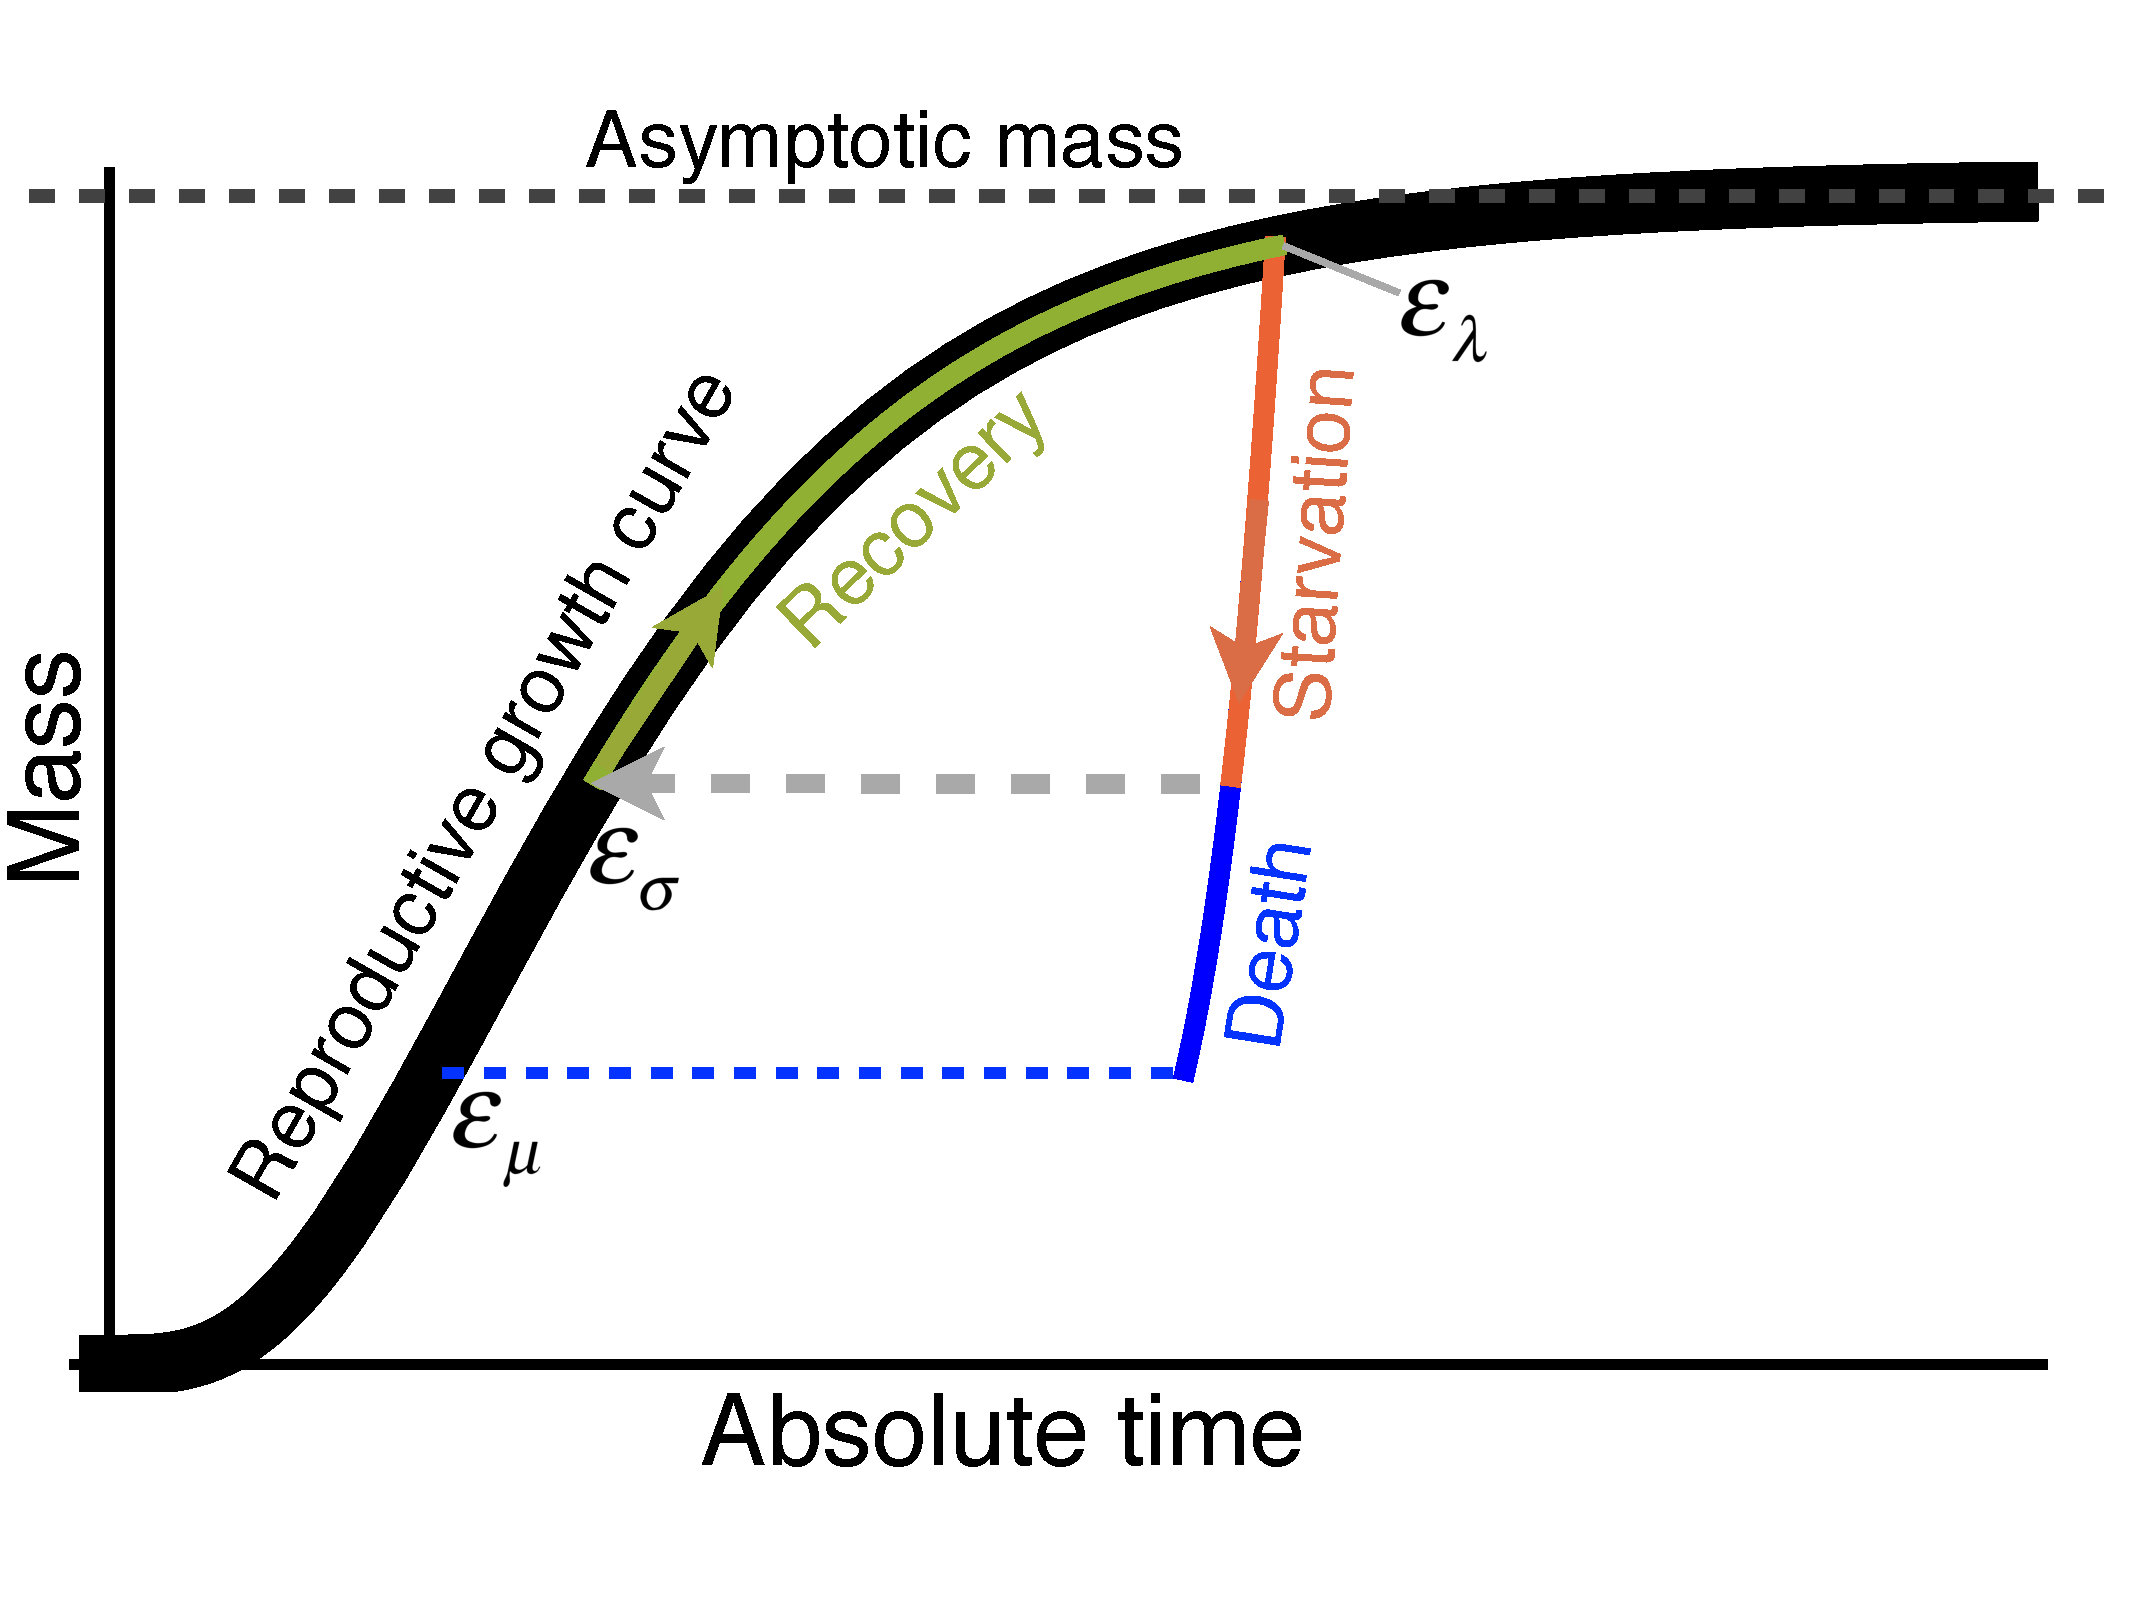
\includegraphics[width=0.5\textwidth]{Growth-trajectory-diagram.pdf}
\caption{
The growth trajectory over absolute time of an individual organism as a function of body mass.
Initial growth follows the red trajectory to an energetically replete adult mass $M$.
Starvation follows the concave blue trajectory to $m_{\rm starve} < M$, whereas recovery follows the convex growth trajectory from $m_\sigma$ to $M$.
}
\label{fig:growth}
\end{figure*}

\begin{figure*}
\centering
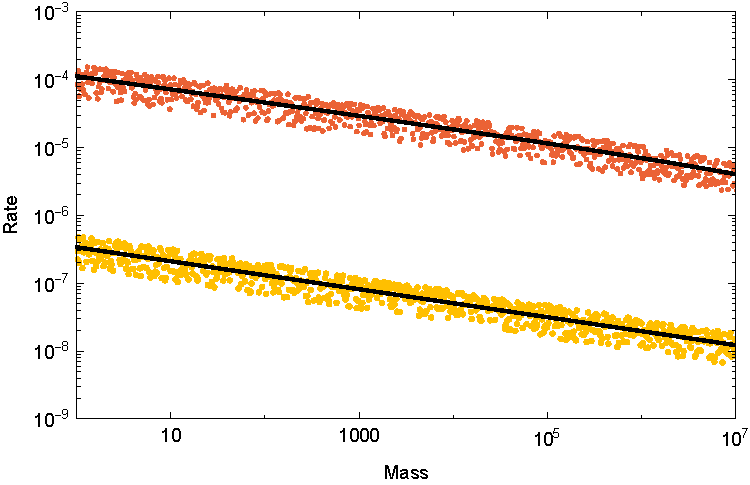
\includegraphics[width=0.5\textwidth]{fig_GvS.pdf}
\caption{
Allometrically constrained starvation rate $\sigma$ (red) vs. reproductive rate $\lambda$ (yellow) as a function of mass $M$.
The rate of starvation is greater than the rate of reproduction for all realized terrestrial endotherm body sizes.
}
\label{fig:gvs}
\end{figure*}

\begin{figure*}
\centering
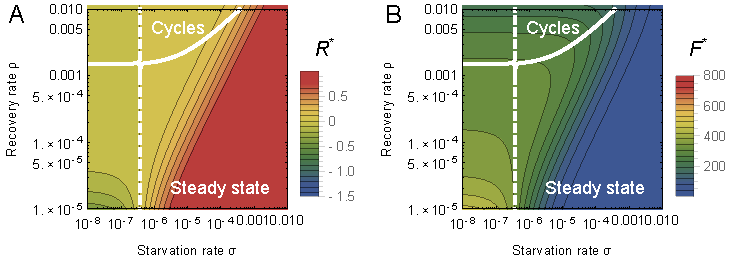
\includegraphics[width=0.5\textwidth]{fig_FixedPoint.pdf}
\caption{
The transcritical (TC; dashed line) and Hopf bifurcation (solid line) as a function of the starvation rate $\sigma$ and recovery rate $\rho$.
These bifurcation conditions separate parameter space into infeasible, cyclic, and steady state dynamic regimes.
The color gradient shows the steady state densities for (A) the resource $R^*$ and the (B) energetically replete consumers $F^*$, with warm colors denoting higher densities and cool colors denoting lower densities.
Steady state densities for the energetically deficient consumers $H^*$ are not shown because they closely mirror those for $F^*$.
}
\label{fig:fp}
\end{figure*}

\begin{figure*}
\centering
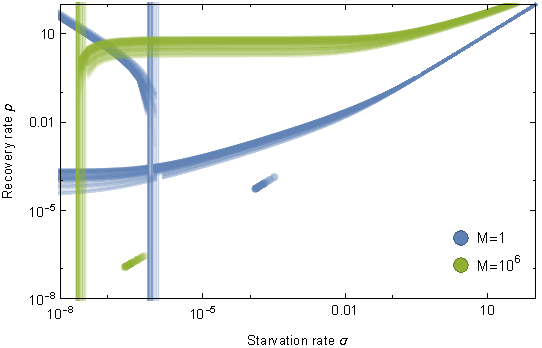
\includegraphics[width=0.5\textwidth]{fig_DataHopf.pdf}
\caption{
Transcritical (TC; vertical lines) and Hopf bifurcations (curved lines) with allometrically determined starvation $\sigma$ and recovery $\rho$ rates as a function of minimum and maximum mammalian body sizes: $1$ gram (blue) and $10^7$ grams (orange), respectively.
Replicates show the influence of variation (20\% around the mean) on allometric parameters, which influences both the energetic rates as well as the position of the TC and Hopf bifurcations.
}
\label{fig:hopf}
\end{figure*}

\begin{figure*}
\centering
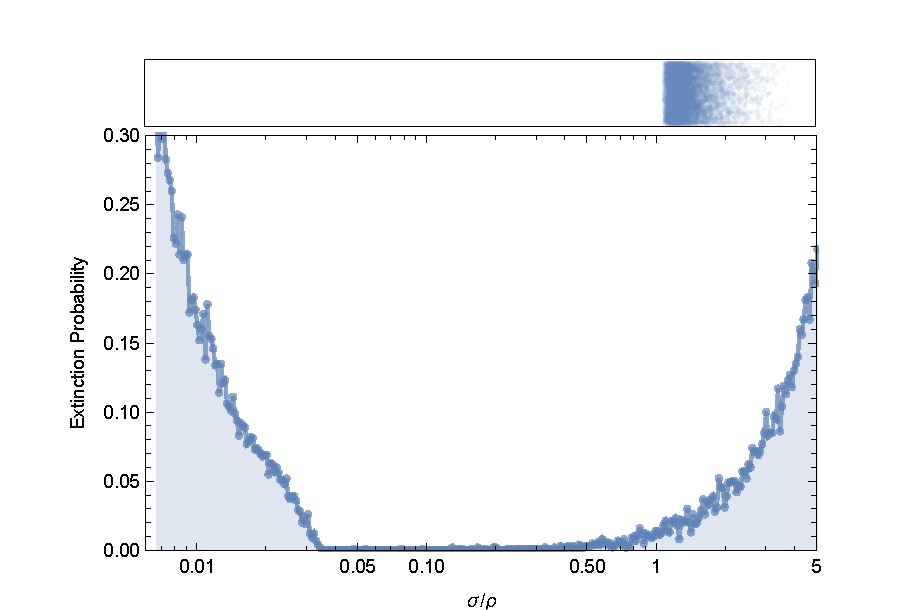
\includegraphics[width=0.5\textwidth]{fig_ExtinctionAllometric.pdf}
\caption{
The probability of extinction for 1000 consumer population trajectories as a function of $\sigma/\rho$ within initial densities chosen to as $A(F^*,H^*,R^*)$, with $A$ a random
variable that is uniformly distribution in $[0,2]$.
Extinction is defined as the population trajectory going below
$0.2~\times$ the allometrically constrained steady state for all times
between $10^2$ and $\leq 10^6$.
The values above the extinction plot are the allometrically constrained $\sigma/\rho$ with 20\% variation around the mean.
}
\label{fig:ext}
\end{figure*} 
 
\begin{figure*}
\centering
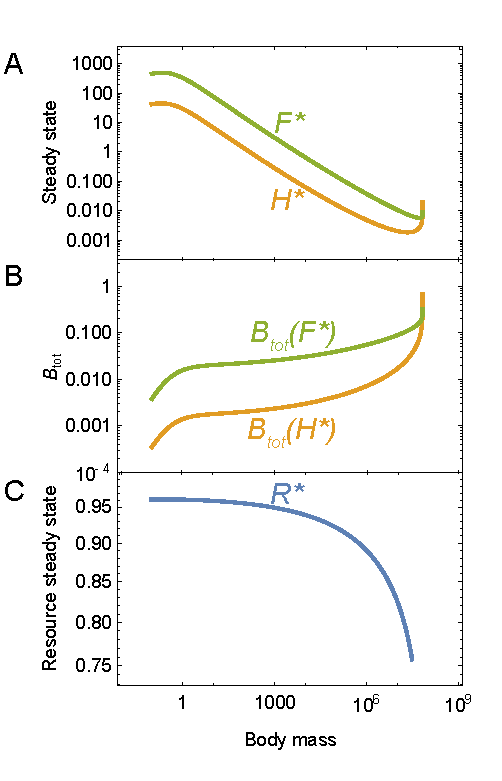
\includegraphics[width=0.45\textwidth]{fig_FPAllometric.pdf}
\caption{
(\emph{A}) Consumer steady states as a function of body size, showing both energetically deficient and replete consumer states ($H^*$ and $F^*$, respectively). 
Energetic rates as a function of body size, with the ratio $\sigma/\rho$ (\emph{B}) and both $\sigma$ (red) and $\rho$ (purple; \emph{C}) drawn separately with 20\% variation around the mean.
Steady state densities decline sharply at $M=M_{\rm min}$ due to the super-exponential decrease in the rate of recovery.
The minimum body size observed for mammals (the Etruscan shrew) is denoted by the orange shaded region at values marking the initial decline of the recovery rate.
}
\label{fig:mass}
\end{figure*}  
 
\begin{figure*}
\centering
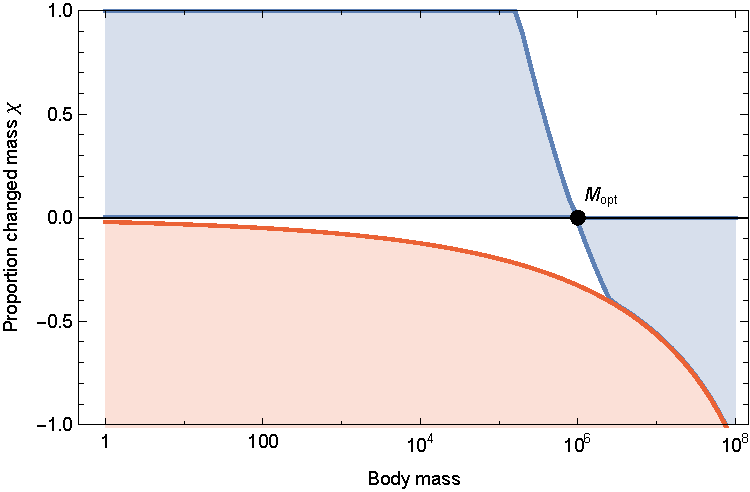
\includegraphics[width=0.5\textwidth]{fig_Invasion.pdf}
\caption{
Invasion feasibility for organisms with a proportional change in mass $\chi$ against a population with a resident body mass $M$.
The blue region denotes which values of $\chi$ result in successful invasion.
The red region denotes which values of $\chi$ result in a mass that is below the starvation threshold and is thus infeasible.
}
\label{fig:invasion}
\end{figure*}  
 

% 
% 
%	 \begin{figure}[h]
%		 \centering
%		 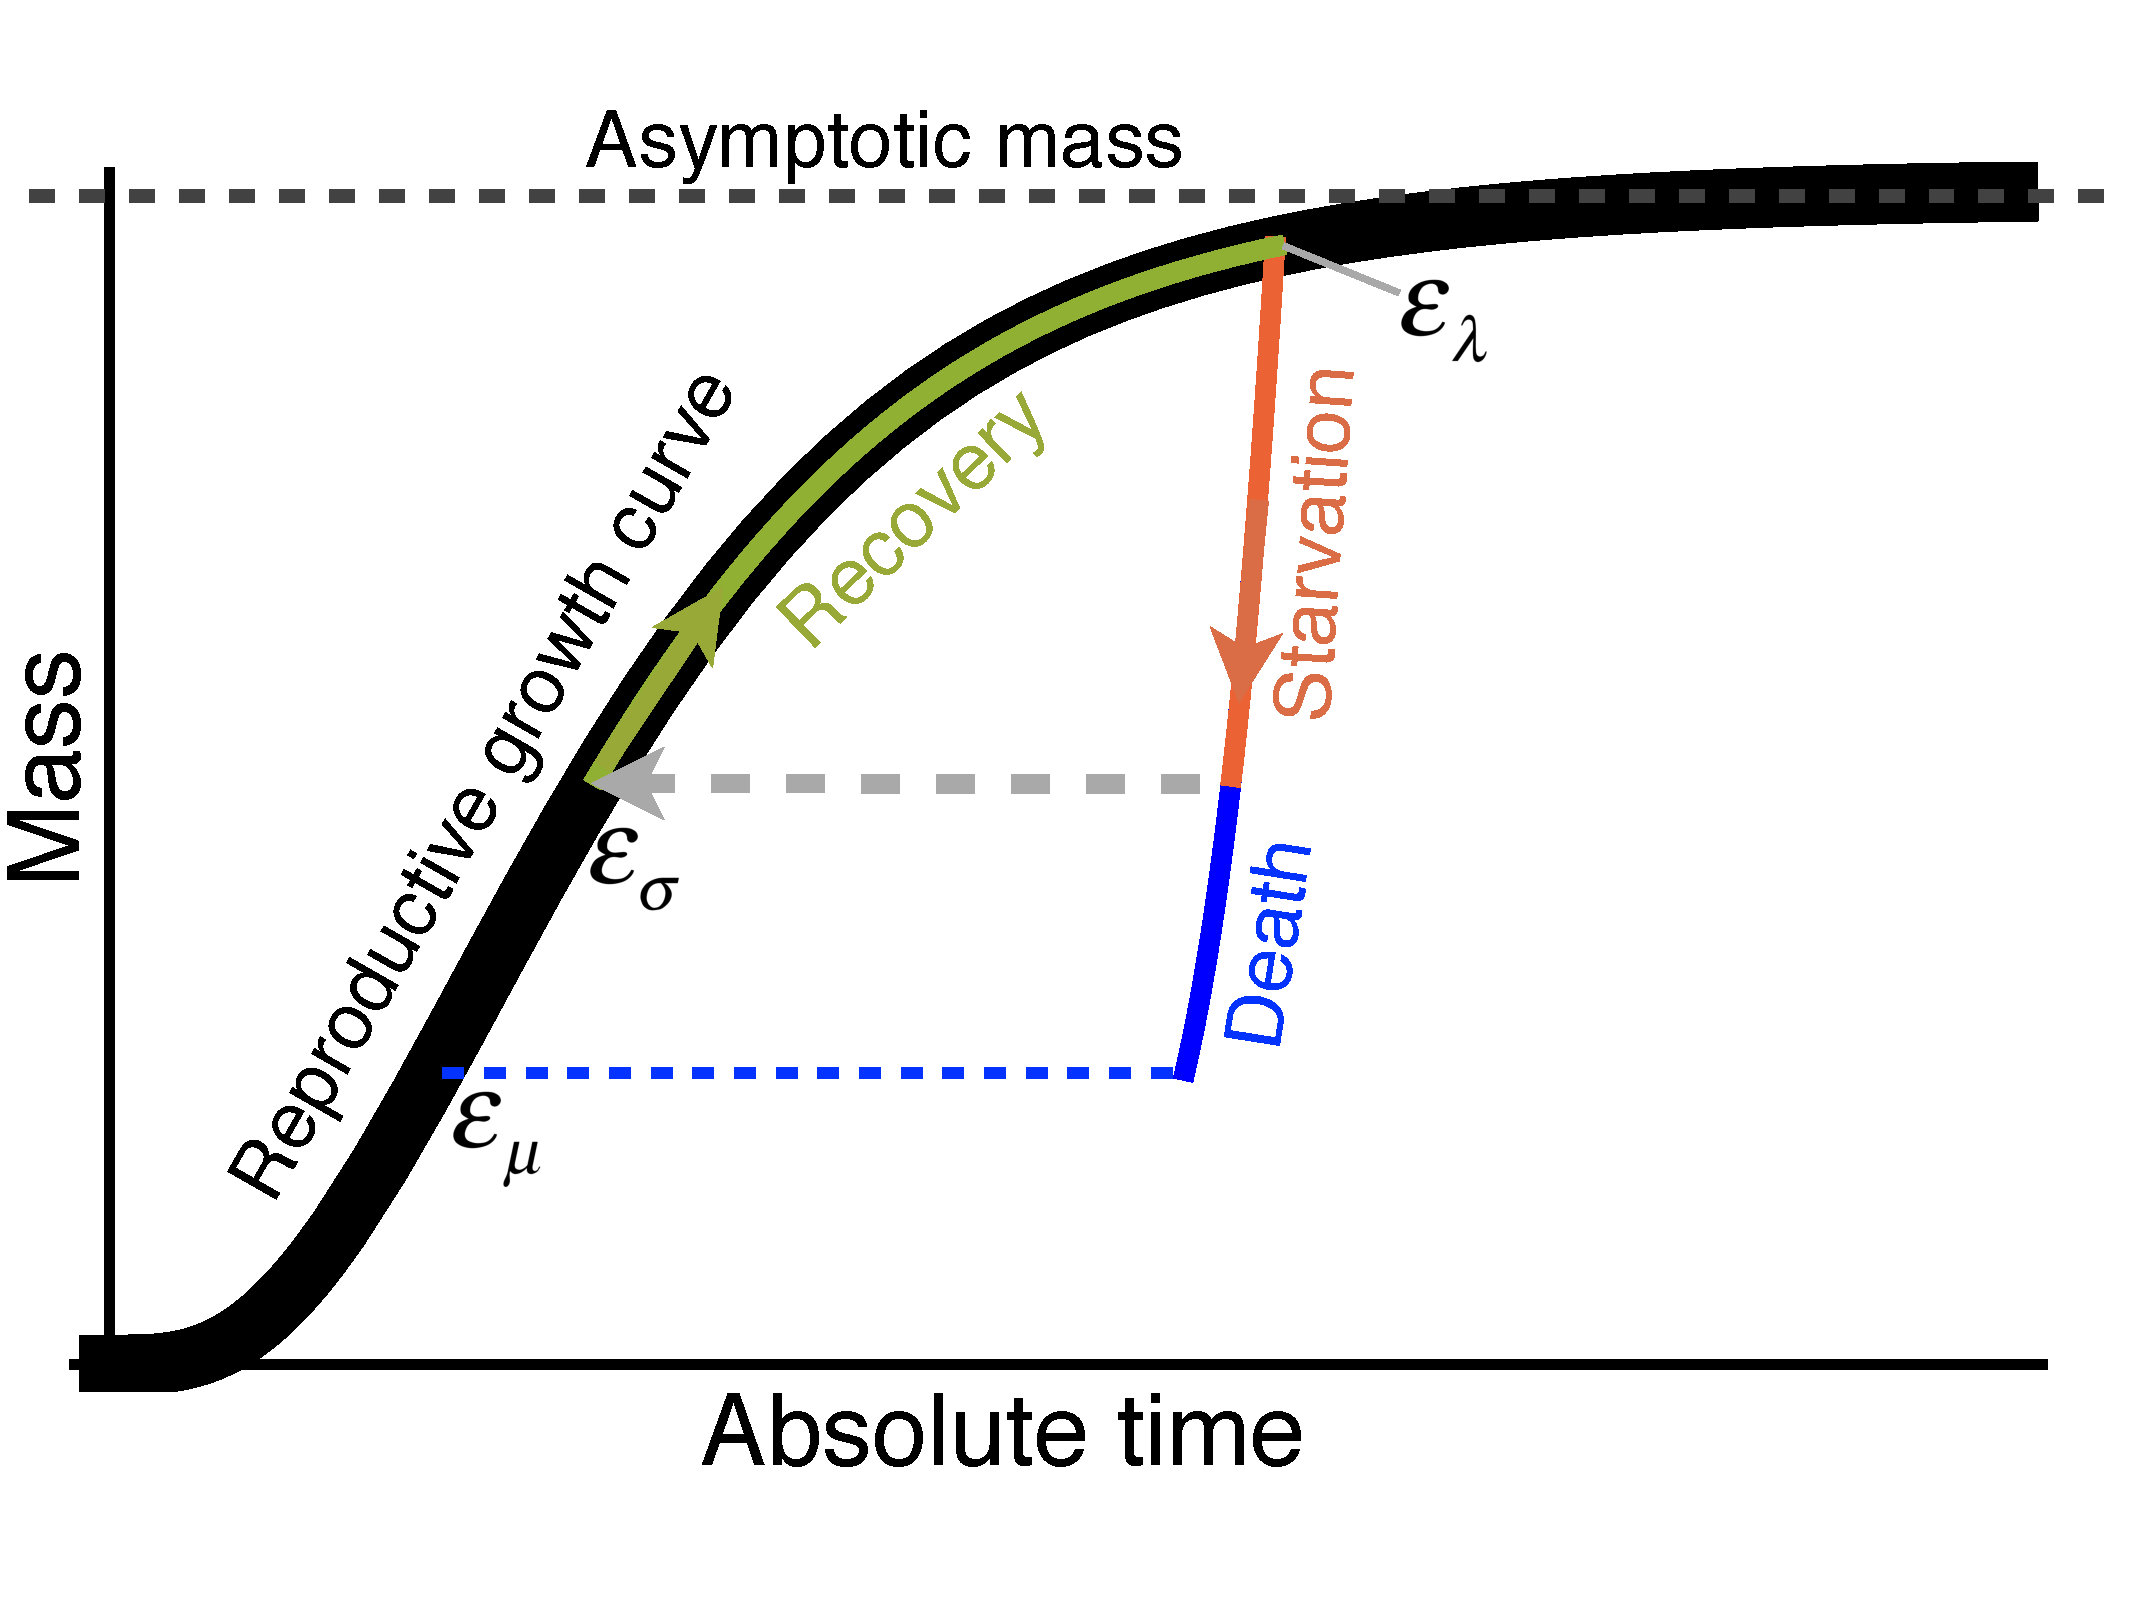
\includegraphics[width=0.5\textwidth]{Growth-trajectory-diagram.pdf}
%		 \caption{
%		 }
%		 \label{growth-diagram}
%	 \end{figure}
%	 
%	 \begin{figure}[h]
%		 \centering
%		 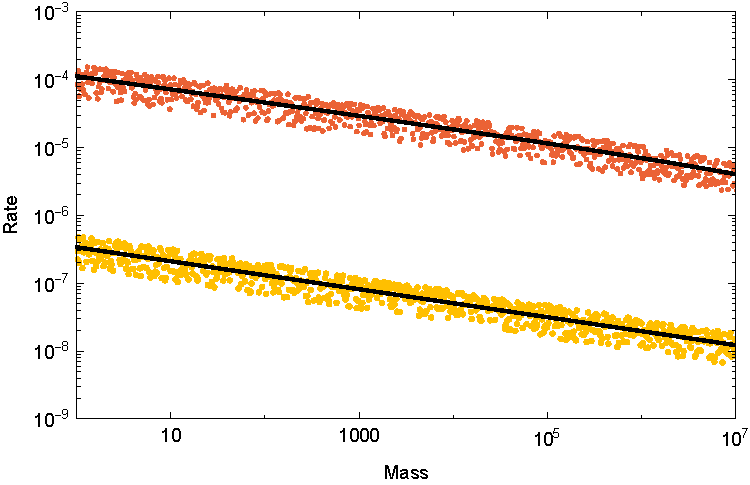
\includegraphics[width=0.25\textwidth]{fig_GvS.pdf}
%		 \caption{
%		 }
%		 \label{GvS}
%	 \end{figure}
%
%
%	\begin{figure}[h]
%	 	\centering
%	 	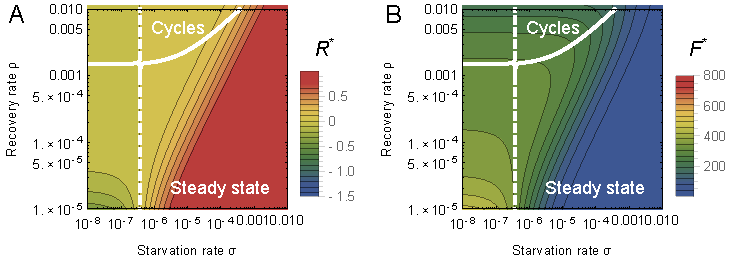
\includegraphics[width=0.25\textwidth]{fig_FixedPoint.pdf}
%	 	\caption{
%	 	}
%		\label{Hopfb}
%	\end{figure}
%
%
%	\begin{figure}[h]
%		\centering
%		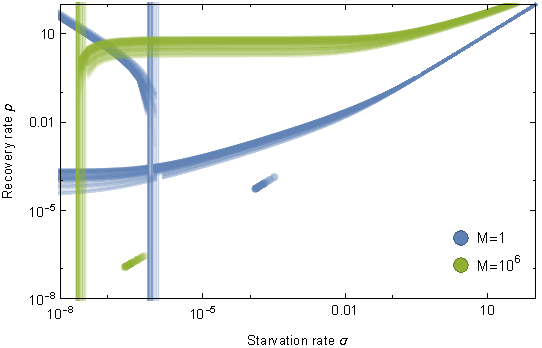
\includegraphics[width=0.8\textwidth]{fig_DataHopf.pdf}
%		\caption{
%		}
%		\label{DataHopf}
%	\end{figure}
%	 
% 
%	\begin{figure}[h]
%		\centering
%	 	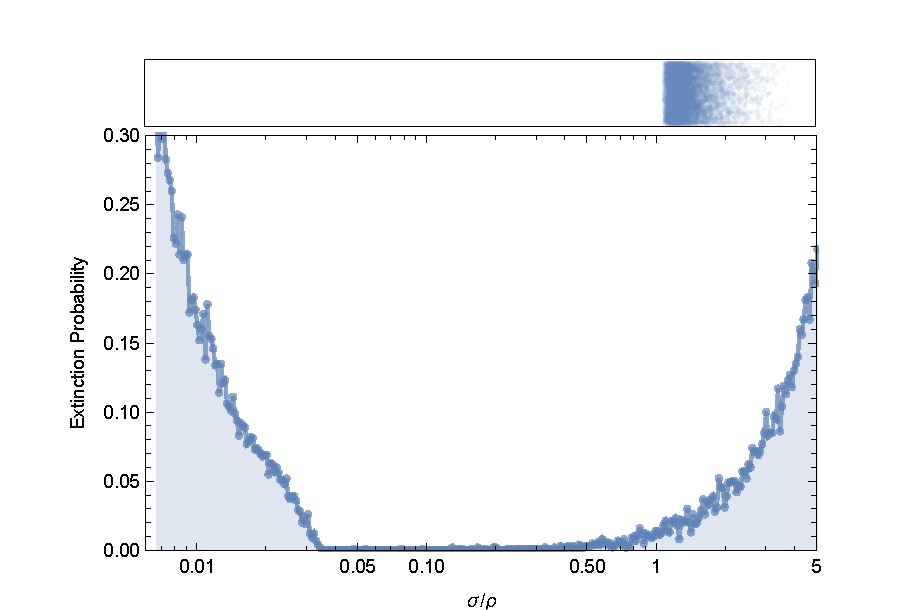
\includegraphics[width=0.8\textwidth]{fig_ExtinctionAllometric.pdf}
%	 	\caption{
%	 	}
%	 	\label{Ext}
%	\end{figure}
%	
%	\begin{figure}[h]
%	 	\centering
%	 	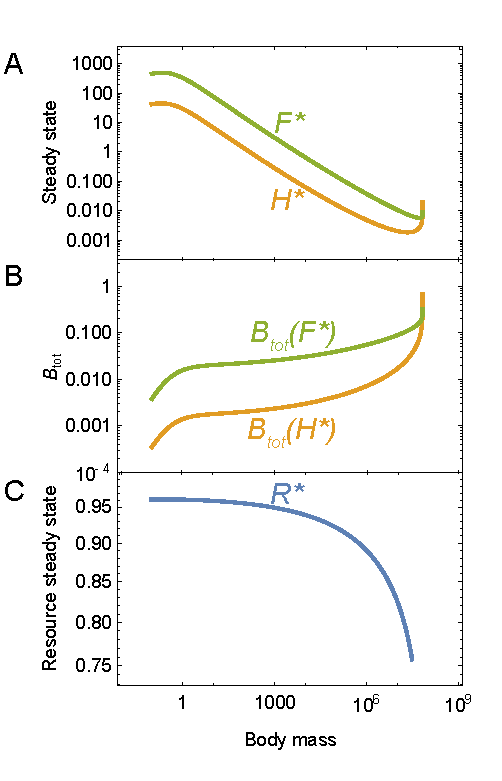
\includegraphics[width=0.5\textwidth]{fig_FPAllometric.pdf}
%	 	\caption{
%	 	}
%	 	\label{Asymp}
%	\end{figure}
%
\clearpage

\begin{table}[h]
\caption{Parameter Values For Various Classes of Organisms}
\label{param}
    \begin{center}
    \small
     \begin{tabular}{| p{1.2cm}| p{3.2cm} | p{2.6cm} | p{3.2cm} | }
     \hline
     & {\bf Mammals} & {\bf Unicellular Eukaryotes} & {\bf Bacteria} \\
     \hline
   $\eta$ & $3/4$ & & $1.70$ \\ 
   $E_{m}$ & $10695$ (J gram$^{-1}$) & & $10695$ (J gram$^{-1}$) \\ 
   $E_{m}^{\prime}$ & $\approx E_{m}$ & & $\approx E_{m}$ \\ 
   $B_{0}$ & $0.019$ (W gram$^{-\alpha}$) & & $1.96\times10^{17}$ \\
   $B_{m}$ & $0.025$ (W gram$^{-1}$)   & & $0.025$ (W gram$^{-1}$)\\
   $a$ & $1.78\times10^{-6}$ & & $1.83\times10^{13}$ \\ 
   $b$ & $2.29\times10^{-6}$ & & $2.29\times10^{-6}$ \\  
   $\eta-1$ & $-0.21$ & & $0.73$ \\ 
   $\lambda_{0}$ & $3.39\times10^{-7}$ (s$^{-1}$ gram$^{1-\eta}$) & & $56493$ \\ 
   $\gamma$ & $1.19$ & & $0.68$ \\ 
   $f_{0}$ & $0.02$ & & $1.30\times10^{-5}$ \\ 
   $\zeta$ & $1.01$ & & \\ 
   $mm_{0}$ & $0.32$ & & \\ 
   
      
   \hline
    \end{tabular}
    \end{center}
   \end{table}



\end{document}






















